% Informe final — Algoritmos y Programación III, 2026-2 (formato IEEE, IEEEtran).
% Compilar:  cd docs/informe/latex && tectonic informe.tex   (figuras: python -m src.evaluation.figuras_informe)
\documentclass[conference,a4paper]{IEEEtran}
\IEEEoverridecommandlockouts

\usepackage[spanish,es-tabla,es-nodecimaldot]{babel}
\usepackage{newtxtext,newtxmath}
\usepackage{amsmath}
\usepackage{graphicx}
\usepackage{booktabs}
\usepackage{multirow}
\usepackage{array}
\usepackage{xcolor}
\usepackage{url}
\usepackage[hidelinks]{hyperref}
\graphicspath{{figuras/}}
\renewcommand{\IEEEkeywordsname}{Palabras clave}
\renewcommand{\arraystretch}{1.08}
\newcommand{\cifra}[1]{\mbox{#1}}

\begin{document}

\title{Clasificación de la calidad y estimación del tamaño de frutas por visión por computador: atajos, fuga de datos y cambio de dominio}

\author{
\IEEEauthorblockN{Juan Manuel Ramírez}
\IEEEauthorblockA{Algoritmos y Programación III\\
Facultad de Ingeniería, Diseño\\ y Ciencias Aplicadas}
\and
\IEEEauthorblockN{Juan Sebastian Poveda}
\IEEEauthorblockA{Algoritmos y Programación III\\
Facultad de Ingeniería, Diseño\\ y Ciencias Aplicadas}
\and
\IEEEauthorblockN{Samuel Jose Rengifo}
\IEEEauthorblockA{Algoritmos y Programación III\\
Facultad de Ingeniería, Diseño\\ y Ciencias Aplicadas}
}

\maketitle

\begin{abstract}
La clasificación manual de fruta fresca es lenta, subjetiva y propensa a errores. Se desarrolló un
sistema que, a partir de una foto de una fruta, predice su calidad (Buena, Defectuosa o Podrida) y
estima su tamaño (Pequeño, Mediano o Grande). El dataset base, FruitNet, solo distingue Good/Bad, por lo
que se re-anotaron 1.200 imágenes y se añadieron dos fuentes públicas y 81 fotos propias como prueba
externa. Se encontraron tres fuentes de métricas infladas: copias aumentadas, sesiones de fotos
repetidas y un fondo que predice la clase (F1 de 0,65 viendo solo el borde de la imagen). Se
corrigieron con particiones por grupos y segmentación U\textsuperscript{2}-Net. Se compararon
regresión logística, SVM y Random Forest sobre 68 rasgos de color, textura y forma, una CNN entrenada
desde cero y EfficientNetB0 con \emph{transfer learning}. La CNN alcanza un F1-macro de 0,91 en
validación y EfficientNetB0 0,85 en prueba, con recall de Podrida de 0,91; con las fotos propias todos
caen a 0,46--0,49, por cambio de dominio y un umbral de pudrición distinto entre fuentes, no por
sobreajuste. El tamaño se mide con una moneda como escala y corrección de perspectiva, con un error
medio de 0,57~cm. La aplicación Streamlit responde en 0,34~s por imagen en CPU.
\end{abstract}

\begin{IEEEkeywords}
calidad de frutas, CNN, \emph{transfer learning}, fuga de datos, cambio de dominio, CRISP-DM
\end{IEEEkeywords}

% ─────────────────────────────────────────────────────────────
\section{Introducción}

En plazas de mercado y agroindustrias la fruta se separa a mano por calidad y tamaño. El proceso es
lento, depende del operario y de su cansancio, y tiene costo: cerca del 14\,\% de los alimentos se
pierde entre la cosecha y la venta minorista \cite{fao2019} y otro 17\,\% se desperdicia en venta y
consumo \cite{unep2021}; las frutas, por perecederas, están entre los productos más afectados. Un
sistema de visión por computador de bajo costo (celular o cámara web más software) puede apoyar esa
inspección, siempre que sea confiable con fruta real y no solo con el dataset de entrenamiento.

\textbf{Objetivo.} Dada una foto de una fruta sobre fondo simple, predecir su calidad en tres clases
---\emph{Buena}, \emph{Defectuosa} (golpes o manchas superficiales; apta con reservas) y \emph{Podrida}
(no apta)--- y estimar su tamaño. Los criterios de éxito, fijados en la primera fase, son: F1-macro
$\geq 0{,}85$; recall de Podrida $\geq 0{,}90$, porque dejar pasar fruta podrida es el error más
costoso; exactitud de tamaño $\geq 0{,}80$, y latencia menor de 1~s por imagen en CPU.

\textbf{Contribuciones.} (i)~Un diagnóstico de tres fuentes de métricas infladas en datasets públicos
de calidad de fruta, con sus correcciones; (ii)~una comparación de ML clásico, CNN desde cero y
\emph{transfer learning} en tres escenarios: mismas fuentes, una fuente no vista y fotos propias;
(iii)~una medición de tamaño con referencia física validada contra regla.

% ─────────────────────────────────────────────────────────────
\section{Fundamentos teóricos}

\textbf{Rasgos diseñados a mano.} El color se resume con histogramas en HSV, que separa el tono (H),
lo que cambia con la pudrición, de la iluminación (V). La textura se describe con patrones binarios
locales (LBP) \cite{ojala2002} y la matriz de co-ocurrencia de grises (GLCM) \cite{haralick1973}, que
capturan manchas, moho y arrugas; la forma, con circularidad, solidez y momentos de Hu.

\textbf{SVM} \cite{cortes1995}. Busca el hiperplano de margen máximo en el espacio inducido por un
núcleo; con el núcleo RBF, $K(\mathbf{u},\mathbf{v})=\exp(-\gamma\lVert\mathbf{u}-\mathbf{v}\rVert^2)$,
separa clases no lineales en el espacio de rasgos.

\textbf{CNN.} Encadena convoluciones que aprenden filtros locales, \emph{pooling} que reduce la
resolución y una capa softmax. \emph{Batch normalization} \cite{ioffe2015} estabiliza el
entrenamiento; se optimiza con Adam \cite{kingma2015} y tasa de aprendizaje con decaimiento coseno
\cite{loshchilov2017}, $\eta_t=\tfrac{\eta_0}{2}\bigl(1+\cos\tfrac{\pi t}{T}\bigr)$.
El \emph{transfer learning} reutiliza una red preentrenada en ImageNet (EfficientNetB0
\cite{tan2019}): primero se entrena una cabeza nueva con la base congelada y luego se ajusta toda la
red con una tasa baja.

\textbf{Aprendizaje por atajos} \cite{geirhos2020}. Una red aprende la regla más fácil que separa las
clases en entrenamiento aunque no sea la causa real ---por ejemplo, el fondo en lugar de la fruta---, y
esa regla deja de funcionar fuera de esa distribución. En \textbf{generalización de dominio}
\cite{gulrajani2021}, entrenar con varias fuentes minimizando el error promedio (ERM) no garantiza
funcionar en una fuente nueva.

% ─────────────────────────────────────────────────────────────
\section{Metodología}

Se siguió CRISP-DM con dos iteraciones (Fig.~\ref{fig:crisp}); cada flecha de retroceso corresponde a
un hallazgo concreto que obligó a volver a una fase anterior.

\begin{figure*}[t]
\centering
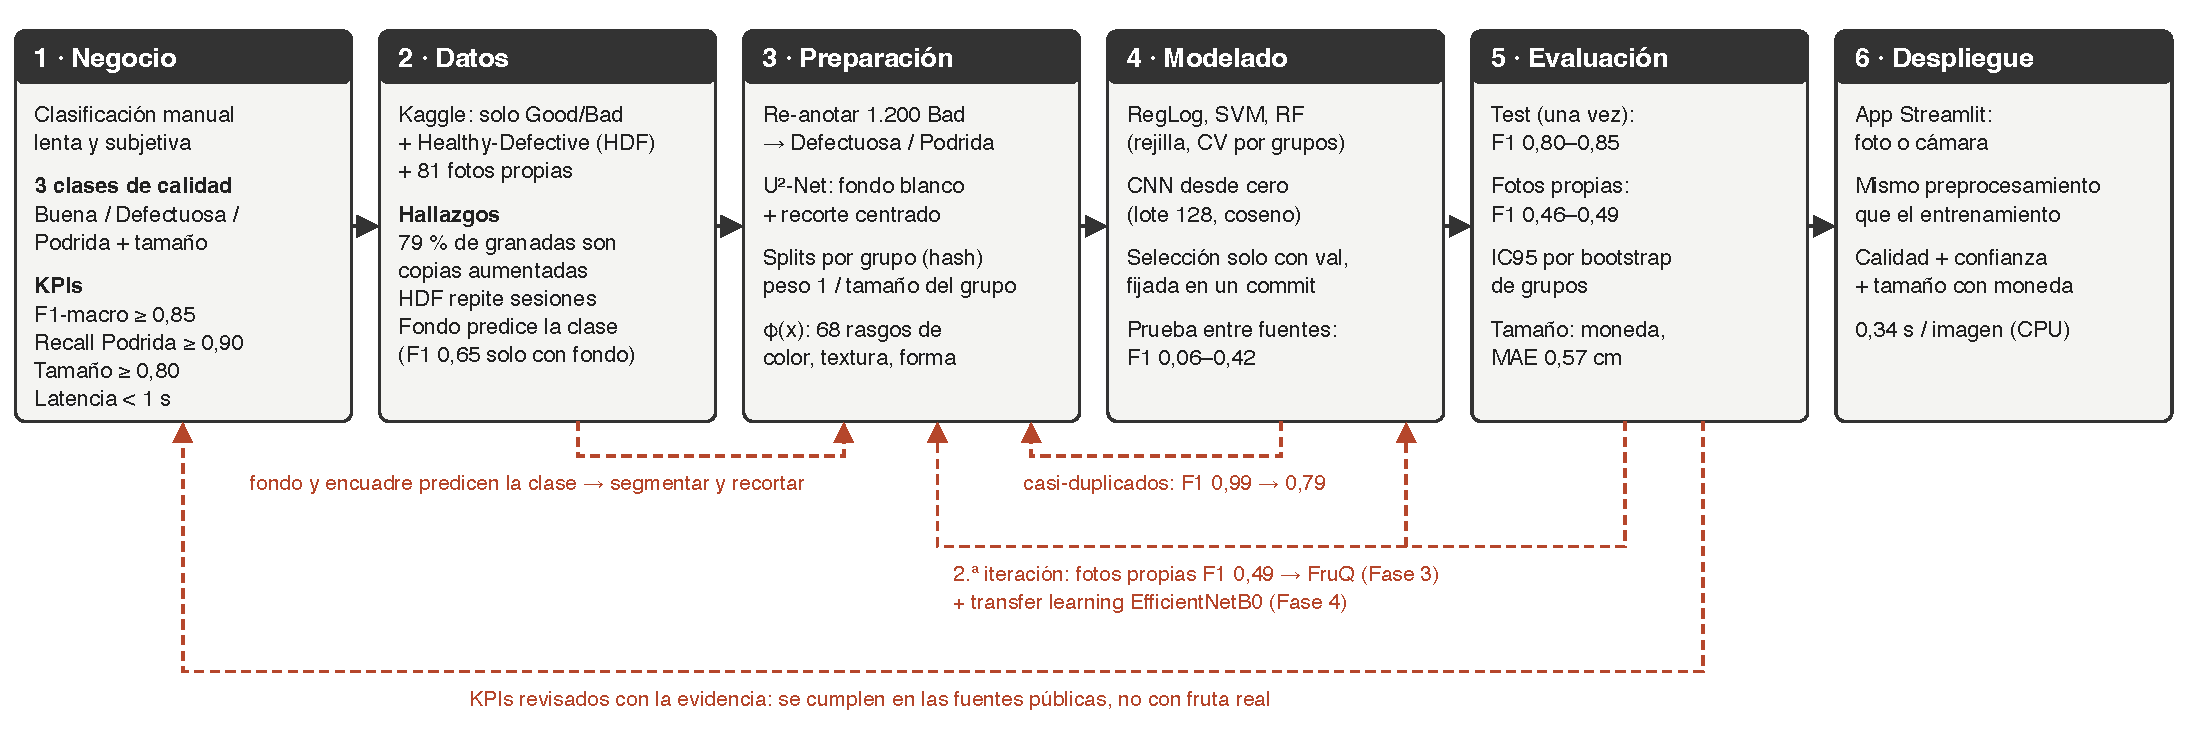
\includegraphics[width=\textwidth]{flujo_crisp_dm.pdf}
\caption{CRISP-DM aplicado al proyecto. Las flechas discontinuas son las iteraciones reales, cada una
motivada por un hallazgo medido.}
\label{fig:crisp}
\end{figure*}

\subsection{Formulación matemática}

Sea $x\in\{0,\dots,255\}^{H\times W\times 3}$ una imagen, $y\in\{1,2,3\}$ su clase de calidad y
$g(x)$ su grupo de origen (misma foto o misma sesión de captura). Se busca $f_\theta$ cuya salida
softmax $p_k=e^{z_k}/\sum_j e^{z_j}$ aproxime $P(y=k\mid x)$, minimizando una entropía cruzada
ponderada por grupo y clase:
\begin{equation}
\begin{aligned}
\mathcal{L}(\theta)&=-\frac{\sum_{i=1}^{N} w_i\log p_{i,y_i}}{\sum_i w_i}+\lambda\lVert\theta\rVert_2^2,\\
w_i&\propto\frac{1}{|g_i|},\qquad \sum_{i:\,y_i=k}w_i=\frac{N}{3}\quad\forall k.
\end{aligned}
\label{eq:loss}
\end{equation}
Con estos pesos, 30 copias de una foto cuentan como una y las tres clases pesan lo mismo; es el único
mecanismo contra el desbalanceo (5:1 entre Buena y el resto). Se descartó SMOTE: interpolar rasgos de
frutas distintas no produce frutas plausibles.

La métrica principal es el F1-macro, $\frac{1}{3}\sum_k 2P_kR_k/(P_k+R_k)$, porque con este
desbalanceo predecir siempre Buena ya da 0,69 de exactitud. La incertidumbre se estima con
\emph{bootstrap} de \emph{grupos} (2.000 remuestreos) \cite{efron1993}: las imágenes de un grupo no
son independientes. Dos modelos se comparan con la diferencia pareada sobre los mismos remuestreos.

\textbf{Tamaño.} Sea $D_m$ el diámetro de la moneda en píxeles. La escala es $s=D_m/26{,}7$~px/mm
(moneda de \$1.000) y la altura de la cámara sale de la focal equivalente $f_{35}$ del EXIF:
$H=f_{35}\,\delta/(43{,}27\,s)$, con $\delta$ la diagonal de la imagen en píxeles. La fruta se modela
como una esfera de radio $r$ apoyada en la mesa; su contorno, visto desde la cámara, corta el plano de
la mesa en una semianchura $a=H\tan\bigl(\arcsin\tfrac{r}{H-r}\bigr)$. Despejando, con
$\sigma=a/\sqrt{H^2+a^2}$,
\begin{equation}
r=\frac{H\,\sigma}{1+\sigma},
\label{eq:size}
\end{equation}
y el diámetro $2r$ se compara con umbrales por fruta $(t_1,t_2)$ tomados de calibres comerciales.

\textbf{Complejidad.} La entrada tiene 49.152 dimensiones; la frontera entre calidades es sutil, no
lineal y subjetiva; hay seis especies con aspecto distinto; los datos esconden fugas y atajos
(§\ref{sec:datos}), y el uso real ocurre en un dominio distinto al de entrenamiento.

\subsection{Datos y hallazgos}\label{sec:datos}

FruitNet \cite{meshram2022} (dataset base exigido) solo trae Good/Bad, y Bad mezcla defectos leves
con pudrición. Se re-anotó con criterios escritos una muestra fija de 1.200 imágenes Bad (200 por
fruta): 842 Podrida, 211 Defectuosa, 13 Buena y 134 descartadas. Healthy-Defective-Fruits (HDF)
\cite{pacheco2023}, del que se usaron solo las imágenes reales de manzana y mango, aporta las tres
clases desde una segunda fuente: si cada clase viniera de una fuente distinta, el modelo aprendería la
fuente y no la calidad. El equipo tomó 81 fotos propias sobre fondo blanco (28 Buena, 23 Defectuosa,
30 Podrida) que se reservaron como prueba externa y nunca se usaron para entrenar ni para elegir
modelos (Tabla~\ref{tab:datos}).

\begin{table}[t]
\caption{Imágenes por fuente y clase (sin las 1.292 en escala de grises)}
\label{tab:datos}
\centering\small
\begin{tabular}{@{}lrrrl@{}}
\toprule
Fuente & Buena & Defect. & Podrida & Uso \\
\midrule
FruitNet \cite{meshram2022} & 10.489 & 211 & 842 & train/val/test \\
HDF \cite{pacheco2023} & 4.909 & 2.987 & 2.000 & train/val/test \\
FruQ \cite{abayomi2023} & 596 & 325 & 594 & solo train (2.ª it.) \\
Propias & 28 & 23 & 30 & prueba externa \\
\bottomrule
\end{tabular}
\end{table}

\textbf{Hallazgo 1: copias aumentadas.} El 79\,\% de las granadas de FruitNet son copias aumentadas de
1.291 fotos únicas; el desbalanceo de granada del análisis exploratorio era artificial. Si una copia
cae en entrenamiento y otra en prueba, la prueba mide memoria.

\textbf{Hallazgo 2: casi-duplicados.} HDF repite la misma fruta o sesión cientos de veces: sus 2.500
manzanas frescas salen de unas 12 sesiones. Con particiones por imagen, el SVM obtenía F1 de 0,99 en
HDF. Al agrupar imágenes con histograma HSV casi idéntico (distancia $L_1<0{,}25$, enlace simple), HDF
pasó de 9.896 a 1.298 grupos y el F1 bajó a 0,79. Los grupos se asignan a train/val/test
($\approx$60/20/20) por un \emph{hash} de su clave, así que al añadir datos ninguna imagen cambia de
partición.

\textbf{Hallazgo 3: el fondo y el encuadre predicen la clase.} Una regresión logística que solo ve un
anillo de 10~px del borde obtuvo F1 de 0,65 (azar: 0,34) y 0,76 en HDF: allí las Buena están
recortadas sobre blanco y las Defectuosa en la mano o en el árbol. U\textsuperscript{2}-Net
\cite{qin2020} separa la fruta, el fondo se reemplaza por blanco y la caja de la fruta se recorta a
128$\times$128 (Fig.~\ref{fig:prep}). Después, el fondo solo da 0,18 y la silueta sin color baja de
0,64 a 0,37 en HDF. El mismo preprocesamiento se usa en la aplicación.

\begin{figure*}[t]
\centering
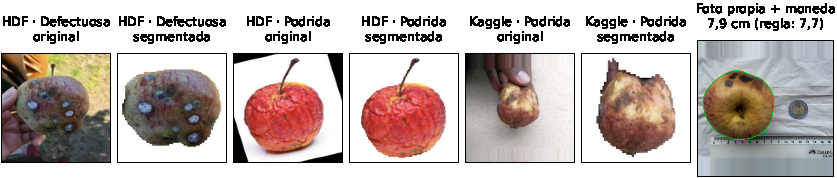
\includegraphics[width=\textwidth]{preparacion.pdf}
\caption{Izquierda: imágenes originales y lo que ven los modelos tras segmentar y recortar (se
eliminan mano, árbol y esquinas de rotación). Derecha: medición de tamaño en una foto propia con la
moneda de \$1.000 (contorno en verde, moneda en azul).}
\label{fig:prep}
\end{figure*}

\subsection{Modelos y selección}

Se entrena con \emph{train} y se elige con \emph{val}; \emph{test} y las fotos propias se abren una sola
vez, con el modelo ya fijado en un \emph{commit}.

\textbf{ML clásico.} El vector $\phi(x)\in\mathbb{R}^{68}$ se calcula solo con los píxeles de la fruta:
color (38), textura LBP+GLCM (18) y forma (12). Se ajustó con \texttt{GridSearchCV} (F1-macro, 5 pliegues
estratificados \emph{por grupo}) y el escalado dentro del \emph{pipeline} para no filtrar estadísticas
de validación. Mejor SVM: RBF, $C=100$, $\gamma=1/(d\,\mathrm{Var}[\phi])$.

\textbf{CNN desde cero} (341 mil parámetros): cuatro bloques [Conv 3$\times$3 $\rightarrow$ BatchNorm
$\rightarrow$ ReLU $\rightarrow$ MaxPool] con 32, 64, 128 y 192 filtros, \emph{global average pooling},
Dense(128), Dropout(0,4) y softmax; el \emph{pooling} global reduce los parámetros de $\sim$4~M a 341
mil. Con lotes de 32 el F1 de validación oscilaba $\pm$0,1 entre épocas: elegir la mejor época era
optimista. La causa era un gradiente ruidoso por los pesos tan desiguales de \eqref{eq:loss}; con
lotes de 128 y tasa coseno la desviación en las últimas 5 épocas bajó a $\pm$0,007. Entrenar sin
aumento de datos fue mejor en dos búsquedas independientes (+0,02 a +0,04, IC95 sin cero).

\textbf{Segunda iteración.} Para atacar la caída con fruta real (§\ref{sec:analisis}) sin tocar las 81
fotos: EfficientNetB0 \cite{tan2019} (3 épocas de cabeza, 15 de ajuste fino desde $10^{-4}$) y FruQ
\cite{abayomi2023}, \emph{time-lapses} de una sola fruta que pasa de fresca a podrida, solo para
entrenar. El criterio, fijado antes de entrenar, fue la validación más una prueba \emph{dejando una
fuente fuera}: entrenar sin Kaggle o sin HDF y validar en la fuente excluida. Se eligió aumento de
color + FruQ.

% ─────────────────────────────────────────────────────────────
\section{Resultados}

Los cinco modelos superan con amplitud la línea base de mayoría (Tabla~\ref{tab:res}). La CNN y
EfficientNetB0 empatan en validación (diferencia pareada $-0{,}00$, IC95 $[-0{,}04;\,+0{,}03]$) y
superan al SVM ($+0{,}07$, IC95 $[+0{,}01;\,+0{,}12]$). La ablación de rasgos del SVM da 0,75 solo con
color, 0,74 solo con textura, 0,56 solo con forma y 0,84 con los tres: color y textura son
complementarios.

\begin{table*}[t]
\caption{F1-macro [IC95 por grupos] y recall de Podrida ($R_P$). Test y fotos propias se evaluaron una sola vez por modelo}
\label{tab:res}
\centering\small
\begin{tabular}{@{}lcccccc@{}}
\toprule
Modelo & Parámetros & Val & Test & $R_P$ test & Fotos propias & $R_P$ propias \\
\midrule
Mayoría & -- & 0,27 & 0,30 & 0,00 & 0,17 & 0,00 \\
Regresión logística & 207 & 0,76 & -- & -- & -- & -- \\
Random Forest & 300 árboles & 0,84 & -- & -- & -- & -- \\
SVM (RBF) & -- & 0,84 [0,73; 0,92] & 0,80 [0,73; 0,87] & 0,81 & 0,46 [0,35; 0,56] & \textbf{0,57} \\
CNN desde cero & 341 mil & \textbf{0,91} [0,85; 0,95] & 0,80 [0,68; 0,93] & \textbf{0,91} & \textbf{0,49} [0,37; 0,59] & 0,27 \\
EfficientNetB0 (TL) & 4,05 M & \textbf{0,91} [0,85; 0,96] & \textbf{0,85} [0,76; 0,94] & \textbf{0,91} & 0,47 [0,36; 0,57] & 0,30 \\
\bottomrule
\end{tabular}
\end{table*}

La Tabla~\ref{tab:fuentes} mide la generalización a una fuente no vista: un SVM entrenado solo con
HDF obtiene 0,06 en Kaggle. El \emph{transfer learning} mejora a la CNN en la fuente no vista, con
diferencia significativa al validar en Kaggle ($+0{,}11$, IC95 $[+0{,}08;\,+0{,}14]$); en HDF el
intervalo es ancho por los pocos grupos.

\begin{table}[t]
\caption{F1-macro en la fuente excluida del entrenamiento}
\label{tab:fuentes}
\centering\small
\begin{tabular}{@{}lcc@{}}
\toprule
Modelo & Kaggle $\rightarrow$ HDF & HDF $\rightarrow$ Kaggle \\
\midrule
SVM & 0,42 & 0,06 \\
CNN desde cero & 0,49 & 0,36 \\
EfficientNetB0 (TL) & \textbf{0,61} & \textbf{0,47} \\
\bottomrule
\end{tabular}
\end{table}

\begin{figure*}[t]
\centering
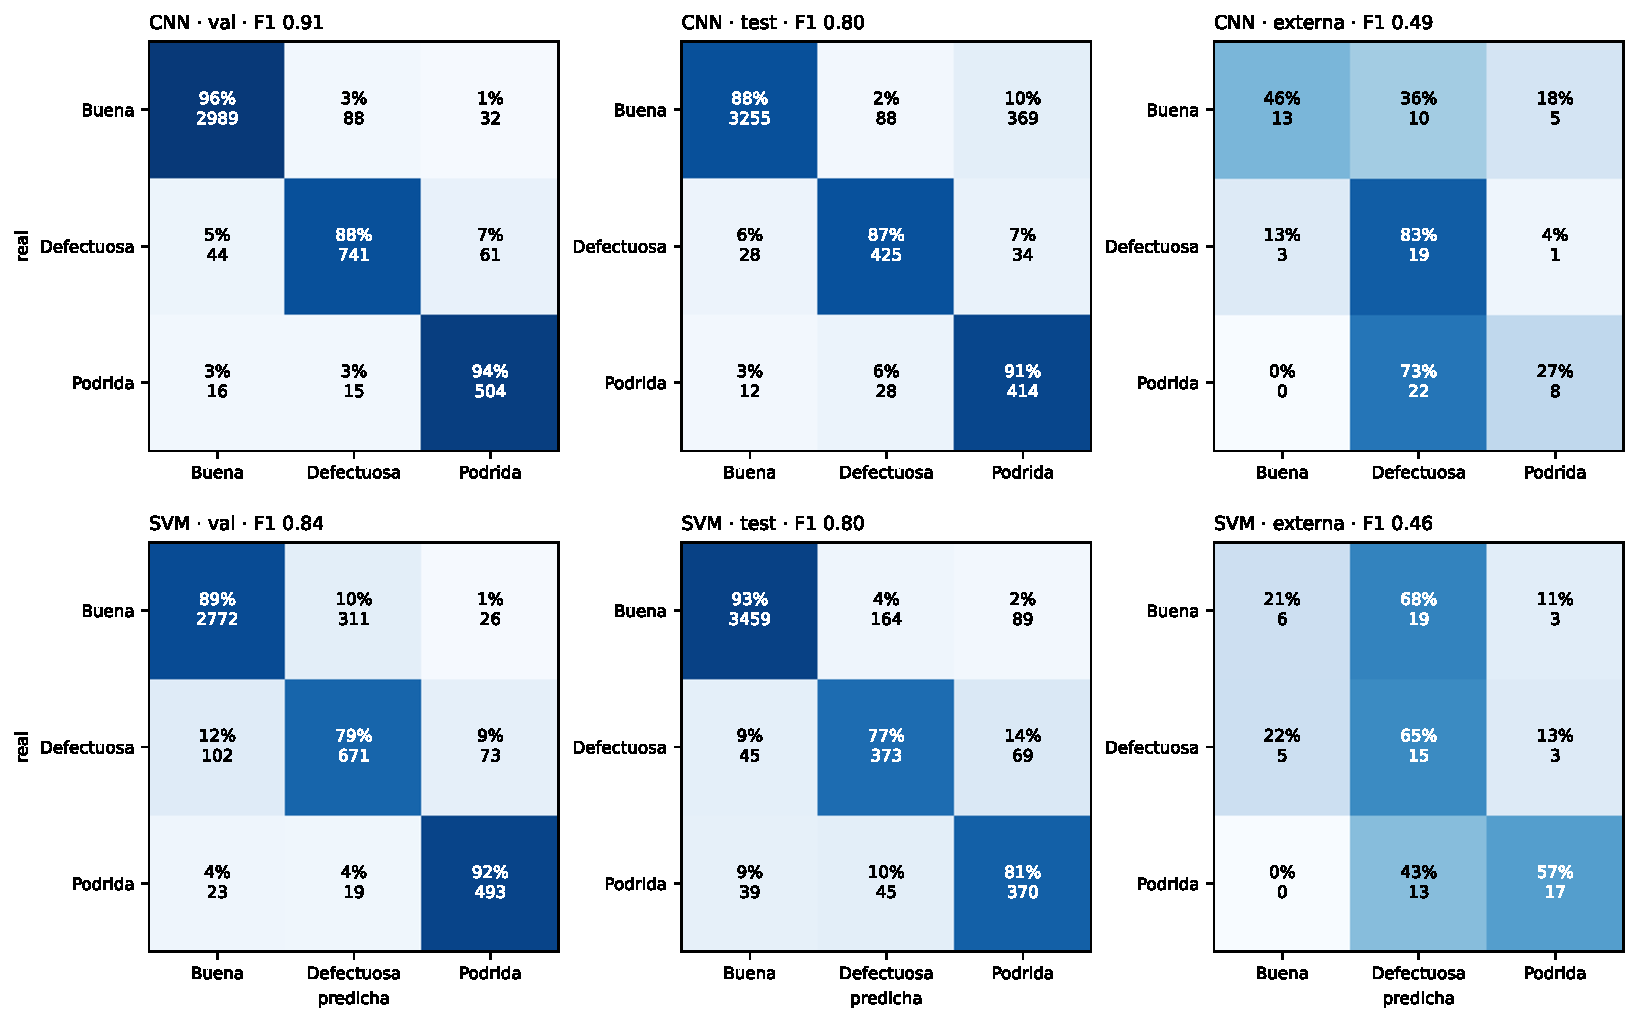
\includegraphics[width=0.78\textwidth]{matrices_confusion.pdf}
\caption{Matrices de confusión de la CNN (arriba) y el SVM (abajo) en validación, test y fotos
propias (externa). Con fruta real ambos empujan casi todo a Defectuosa.}
\label{fig:cm}
\end{figure*}

\textbf{Tamaño.} En 11 frutas medidas con regla (7 limones, 3 manzanas, 1 naranja; iPhone a 20--29~cm),
la moneda se detectó en todas y su escala coincide con la de una regla visible en cada foto (2--3\,\%).
El error medio absoluto del diámetro es 0,57~cm (sesgo $+0{,}38$~cm) y la clase de tamaño es correcta
en 5 de 11. Una primera versión medía el ancho máximo, que incluye las puntas del limón y el pedúnculo,
y daba 1,10~cm; se cambió al diámetro ecuatorial, el calibre de las normas comerciales
\cite{codex2010}.

\textbf{Latencia.} 0,34~s por imagen en CPU (Apple M4) con EfficientNetB0, incluida la segmentación;
0,37~s con la medición de tamaño.

% ─────────────────────────────────────────────────────────────
\section{Análisis de resultados}\label{sec:analisis}

\textbf{¿Sobreajuste?} No en las redes: la CNN obtiene 0,91 en \emph{train} y 0,91 en \emph{val},
porque los pesos por grupo impiden memorizar sesiones repetidas. El SVM sí memoriza (1,00 frente a
0,84), efecto que acota la validación cruzada por grupos.

\textbf{De validación a test (0,91$\rightarrow$0,80 en la CNN).} No es sobreajuste: 306 de los 369
errores Buena$\rightarrow$Podrida provienen de una sola sesión de HDF, manzanas Red Delicious de rojo muy
oscuro que la red asocia con pudrición. Contando cada fruta una vez (métrica decidida después de ver
test, solo como diagnóstico), la CNN vuelve a 0,90. EfficientNetB0, preentrenada con millones de
imágenes naturales, reduce esos errores de 358 a 66; es su única mejora clara en test.

\textbf{Fotos propias (F1$\approx$0,47 en los tres modelos).} La CNN y EfficientNetB0 coinciden en el
62\,\% de las fotos y fallan juntas en el 35\,\%; con arquitecturas tan distintas, esto indica que el
límite está en los datos y no en el modelo. El error dominante es el más costoso, Podrida
$\rightarrow$ Defectuosa (20 de 30, Fig.~\ref{fig:cm}): 12 son manzanas con manchas marrones moderadas,
en la frontera de nuestro criterio y más leves que las Podrida de HDF, y 5 son naranjas con moho, un
caso casi ausente en entrenamiento. Las causas son el \emph{cambio de dominio} (variedad, cámara y luz),
coherente con la Tabla~\ref{tab:fuentes}, y un \emph{umbral de pudrición distinto} entre las fuentes
públicas y nuestro criterio; ninguna se corrige con más capacidad del modelo. Como detector de fruta
dañada frente a buena, EfficientNetB0 detecta 49 de las 53 dañadas, pero acierta solo 13 de las 28
Buena: serviría como primer filtro con revisión humana, no como clasificador autónomo.

\textbf{Comparación con la literatura.} Con FruitNet, Morshed \emph{et~al.} \cite{morshed2022}
reportan 99,67\,\% de exactitud en 3 niveles de calidad con una partición 60:20:20 cuyo método no se
detalla, sin mencionar las copias aumentadas. Pacheco \emph{et~al.} \cite{pacheco2023} reportan
97,5\,\% en manzanas de HDF con MobileNetV2. Nuestras cifras no son directamente comparables: con
partición por imagen, nuestro SVM también llegaba a 0,96 global y 0,99 en HDF, y al agrupar copias y
sesiones bajó a 0,84 y 0,79. Esto no prueba que esos trabajos tengan fuga, pero muestra que en estos
datasets \emph{la forma de partir los datos cambia el resultado más que la arquitectura}. La falla
entre fuentes coincide con \cite{gulrajani2021}, y el atajo de fondo es un caso concreto de
\cite{geirhos2020}.

\textbf{Tamaño.} El error no viene de la escala, que coincide con la regla en 2--3\,\%. Es del orden
del ancho de los rangos de limón (1~cm), así que una fruta cerca de un umbral se clasifica mal con
facilidad; además, las medidas con regla son ruidosas (un limón anotado en 3,8~cm se ve más grande que
otro de 4,5~cm), y el cambio a diámetro ecuatorial se decidió viendo estas 11 frutas, por lo que el
0,57~cm es optimista. No se entrenó un modelo de tamaño: una foto sin referencia no tiene escala
absoluta y ningún dataset trae tamaños reales, así que una medición geométrica con referencia física
es más defendible.

% ─────────────────────────────────────────────────────────────
\section{Ética e impactos}

Las decisiones se relacionan con el Código de Ética de la ACM \cite{acm2018}
(Tabla~\ref{tab:etica}); la Tabla~\ref{tab:impactos} resume los impactos y su mitigación.

\textbf{Honestidad en la evaluación.} El dilema más concreto del proyecto no fue hipotético: las
métricas fáciles de obtener (F1 de 0,96--0,99 con partición por imagen, o la mejor época elegida con
la propia validación) eran las más favorables y las menos ciertas. El principio 2.5 de la ACM pide
evaluaciones completas que incluyan sus riesgos; por eso se fijó cada modelo en un \emph{commit} antes
de abrir test, se reportan intervalos por grupos y se declara que la cifra con fruta real es 0,47.
Publicar 0,91 como desempeño del sistema habría inducido a usarlo donde falla.

\textbf{Daño asimétrico y supervisión humana.} Los dos errores no cuestan lo mismo: Podrida
$\rightarrow$ Buena puede llegar al consumidor (principio 1.2), mientras que Buena $\rightarrow$
Dañada es merma para el vendedor. El KPI de recall de Podrida prioriza el primero, y con fruta real el
error dominante va hacia Defectuosa y no hacia Buena (0 de 30 Podrida predichas como Buena por la
CNN), lo que es el fallo menos dañino. Aun así, con F1 de 0,47 el sistema solo es defendible como apoyo:
la app muestra la confianza y la decisión queda en manos del operario, lo que también atenúa el
impacto laboral (principio 1.1).

\textbf{Sesgo de dominio como problema de equidad.} Las fuentes públicas vienen de India y Ecuador; con
fruta y variedades locales el modelo empeora (manzanas rayadas tipo Gala marcadas como dañadas). Un
mercado pequeño que lo adopte sin datos propios recibiría peor servicio que el dataset de origen; la
mitigación es recolectar y validar con fruta local y reportar el desempeño por dominio, no solo el
global (principio 1.4).

\begin{table*}[t]
\caption{Dilemas éticos, principio del código de ética de la ACM y medida adoptada}
\label{tab:etica}
\centering\footnotesize
\begin{tabular}{@{}p{3.2cm}p{3.4cm}p{2.6cm}p{7.2cm}@{}}
\toprule
Situación & Dilema & Principio ACM & Medida adoptada \\
\midrule
Fotos propias en casa y mercado & Privacidad; captura de personas & 1.6 Privacidad & Solo la fruta sobre fondo blanco, sin personas; las 104 fotos versionadas no tienen GPS en el EXIF (verificado) \\
Datasets de terceros & Atribución y licencias & 1.5 Reconocer el trabajo ajeno & Fuentes y código citados; HDF y FruQ (CC~BY~4.0) con atribución; el repositorio solo versiona fotos propias \\
Métricas infladas (copias, atajos) & Reportar la cifra que favorece al proyecto & 1.3 Honestidad; 2.5 Evaluación completa & Particiones por grupo; test abierto una sola vez con el modelo fijado; se reporta F1 0,47 con fruta real \\
Error Podrida $\rightarrow$ Buena & Riesgo para el consumidor & 1.2 Evitar daño & KPI de recall de Podrida; la app muestra la confianza; uso como filtro con revisión humana \\
Sesgo por variedad y fuente & Peor desempeño con fruta local & 1.4 Equidad & Análisis por fuente y por fruta; limitación declarada \\
Automatizar la clasificación & Desplazamiento laboral & 1.1 Bienestar social & Herramienta asistiva: el operario decide \\
Etiquetas subjetivas & Criterio de un solo anotador & 2.5 Evaluación completa & Criterios escritos; kappa de Cohen \cite{cohen1960} entre anotadores \textcolor{red}{[pendiente]} \\
\bottomrule
\end{tabular}
\end{table*}

\begin{table*}[t]
\caption{Matriz de impactos y estrategias de mitigación}
\label{tab:impactos}
\centering\footnotesize
\begin{tabular}{@{}p{1.7cm}p{4.2cm}p{5.0cm}p{5.5cm}@{}}
\toprule
Dimensión & Impacto positivo & Riesgo & Mitigación \\
\midrule
Social & Criterio uniforme; menos trabajo repetitivo & Confianza excesiva en un modelo que falla con fruta real & Mostrar la confianza; revisión humana de casos dudosos \\
Económica & Menos merma por fruta buena descartada & Descartar fruta buena (15 de 28 Buena propias marcadas como dañadas) & Calibrar con fotos locales antes de usar \\
Ambiental & Menos desperdicio de alimentos \cite{fao2019,unep2021} & Energía de la inferencia & Modelos pequeños (341 mil parámetros); inferencia en CPU, sin GPU \\
Global & Herramienta barata para mercados pequeños & Datasets de otras regiones (India, Ecuador) & Recolectar datos locales; reportar el desempeño por dominio \\
\bottomrule
\end{tabular}
\end{table*}

% ─────────────────────────────────────────────────────────────
\section{Conclusiones y trabajo futuro}

Se construyó un sistema completo, de los datos a la aplicación, para clasificar la calidad de fruta en
tres clases y estimar su tamaño. Dentro de las fuentes públicas, la CNN desde cero y EfficientNetB0
alcanzan F1-macro de 0,91 en validación y 0,80--0,85 en test, con recall de Podrida de 0,91: cumplen
el KPI de recall, y EfficientNetB0 el de F1 en test. Con fruta real los tres enfoques caen a
F1$\approx$0,47 y no son aptos para uso autónomo.

Lo aprendido: en datasets públicos de calidad de fruta, copias, casi-duplicados y fondos
correlacionados inflan las métricas, y la partición por grupos y una prueba externa son
indispensables. Elegir la arquitectura importa menos que el dominio y el criterio de etiquetado: el
\emph{transfer learning} mejora la generalización entre fuentes, pero no cierra la brecha con fruta
real. La medición de tamaño con moneda tiene un error de 0,57~cm, aunque la clase de tamaño no alcanza
el KPI (5/11) por umbrales sin calibrar y medidas de referencia ruidosas.

Trabajo futuro, por impacto esperado: (1)~fotografiar más fruta local y usar parte para ajustar el
modelo; (2)~alinear el umbral Defectuosa/Podrida de las fuentes públicas con el criterio propio;
(3)~añadir ejemplos de moho en cítricos; (4)~una salida de rechazo para imágenes fuera de dominio;
(5)~calibrar los umbrales de tamaño con frutas medidas con calibrador, y (6)~medir el acuerdo entre
anotadores.

% ─────────────────────────────────────────────────────────────
\begin{thebibliography}{20}
\footnotesize

\bibitem{fao2019} FAO, \emph{The State of Food and Agriculture 2019: Moving Forward on Food Loss and Waste Reduction}. Roma, Italia: FAO, 2019.

\bibitem{unep2021} UNEP, \emph{Food Waste Index Report 2021}. Nairobi, Kenia: United Nations Environment Programme, 2021.

\bibitem{meshram2022} V.~Meshram y K.~Patil, ``FruitNet: Indian fruits image dataset with quality for machine learning applications,'' \emph{Data in Brief}, vol.~40, art.~107686, 2022, doi: 10.1016/j.dib.2021.107686.

\bibitem{pacheco2023} R.~Pacheco, P.~González, L.~Chuquimarca, B.~Vintimilla y S.~Velastin, ``Fruit defect detection using CNN models with real and virtual data,'' en \emph{Proc. 18th Int. Joint Conf. Computer Vision, Imaging and Computer Graphics Theory and Applications (VISAPP)}, 2023, pp.~272--279, doi: 10.5220/0011679800003417.

\bibitem{abayomi2023} O.~O. Abayomi-Alli, R.~Damaševičius, S.~Misra y A.~Abayomi-Alli, ``FruitQ: a new dataset of multiple fruit images for freshness evaluation,'' \emph{Multimedia Tools and Applications}, 2023, doi: 10.1007/s11042-023-16058-6.

\bibitem{qin2020} X.~Qin, Z.~Zhang, C.~Huang, M.~Dehghan, O.~R. Zaiane y M.~Jagersand, ``U\textsuperscript{2}-Net: Going deeper with nested U-structure for salient object detection,'' \emph{Pattern Recognition}, vol.~106, art.~107404, 2020.

\bibitem{tan2019} M.~Tan y Q.~V. Le, ``EfficientNet: Rethinking model scaling for convolutional neural networks,'' en \emph{Proc. 36th Int. Conf. Machine Learning (ICML)}, 2019, pp.~6105--6114.

\bibitem{ioffe2015} S.~Ioffe y C.~Szegedy, ``Batch normalization: Accelerating deep network training by reducing internal covariate shift,'' en \emph{Proc. 32nd Int. Conf. Machine Learning (ICML)}, 2015, pp.~448--456.

\bibitem{kingma2015} D.~P. Kingma y J.~Ba, ``Adam: A method for stochastic optimization,'' en \emph{Proc. Int. Conf. Learning Representations (ICLR)}, 2015.

\bibitem{loshchilov2017} I.~Loshchilov y F.~Hutter, ``SGDR: Stochastic gradient descent with warm restarts,'' en \emph{Proc. Int. Conf. Learning Representations (ICLR)}, 2017.

\bibitem{geirhos2020} R.~Geirhos \emph{et~al.}, ``Shortcut learning in deep neural networks,'' \emph{Nature Machine Intelligence}, vol.~2, pp.~665--673, 2020.

\bibitem{gulrajani2021} I.~Gulrajani y D.~Lopez-Paz, ``In search of lost domain generalization,'' en \emph{Proc. Int. Conf. Learning Representations (ICLR)}, 2021.

\bibitem{morshed2022} M.~S. Morshed, S.~Ahmed, T.~Ahmed, M.~U. Islam y A.~B.~M.~A. Rahman, ``Fruit quality assessment with densely connected convolutional neural network,'' arXiv:2212.04255, 2022.

\bibitem{cortes1995} C.~Cortes y V.~Vapnik, ``Support-vector networks,'' \emph{Machine Learning}, vol.~20, no.~3, pp.~273--297, 1995.

\bibitem{ojala2002} T.~Ojala, M.~Pietikäinen y T.~Mäenpää, ``Multiresolution gray-scale and rotation invariant texture classification with local binary patterns,'' \emph{IEEE Trans. Pattern Anal. Mach. Intell.}, vol.~24, no.~7, pp.~971--987, 2002.

\bibitem{haralick1973} R.~M. Haralick, K.~Shanmugam e I.~Dinstein, ``Textural features for image classification,'' \emph{IEEE Trans. Syst., Man, Cybern.}, vol.~SMC-3, no.~6, pp.~610--621, 1973.

\bibitem{cohen1960} J.~Cohen, ``A coefficient of agreement for nominal scales,'' \emph{Educational and Psychological Measurement}, vol.~20, no.~1, pp.~37--46, 1960.

\bibitem{efron1993} B.~Efron y R.~J. Tibshirani, \emph{An Introduction to the Bootstrap}. Nueva York, NY, EE.~UU.: Chapman \& Hall, 1993.

\bibitem{codex2010} Codex Alimentarius, \emph{Standard for Apples}, CXS 299-2010. Roma, Italia: FAO/OMS, 2010.

\bibitem{acm2018} ACM, \emph{ACM Code of Ethics and Professional Conduct}, 2018. [En línea]. Disponible: \url{https://www.acm.org/code-of-ethics}

\end{thebibliography}

\end{document}
